\section{Analysis Strategy}
%%%%%%%%%%%%%%%%%%%%%%%%%%%%%%%%%%%%%%%%%%%%%%%%%%%%%%%%%%%%%%%%%%%%%%
\label{sec:AnalysisStrategy}

The analysis presented here is based on that used in the previously published \hwwllnn{}
measurements by CMS~\cite{Chatrchyan:2013iaa}, modified to be inclusive in the number of jets. 
This modification significantly reduces the uncertainties related to the modelling of the number of jets produced in association with the Higgs boson.


\subsection{Event reconstruction and selections}\label{sec:Selections}

%%% Physics objects definition
The electron selection is based on two multivariate discriminants, one specialised in identifying the electron object and the other for isolation. The cut value for each discriminant is optimised to provide a good fake electron rejection and to improve the signal acceptance.

Muons are reconstructed using the standard CMS selection and are required to be identified both in the tracker (\textit{tracker muon}) and in the muon chambers (\textit{global muon}). Additionally quality criteria on the muon track are required, such as to have at least 10 hits in the tracker (at least one of which in the pixel detector) and to have $\chi^2/ndf < 10$.
Muon isolation is based on the Particle-Flow algorithm. An MVA approach is considered, based on the radial distributions of the Particle-Flow candidates inside a cone of radius 0.5 around the muon direction.

The efficiencies for the identification and isolation of the electrons and muons are measured in data and in simulation selecting a pure sample of leptons coming from the Z$\to\ell\ell$ decay. The measured efficiencies are used as scale factors to correct the MC simulation to precisely model the data. Similarly, the trigger efficiency extracted fromdata is applied toMC samples to correct for the additional loss.

Jets in this analysis are reconstructed by combining the energy measured in the calorimeters and tracks from charged particles on basis of the standard CMS particle flow algorithm and using the anti-$k_T$ clustering algorithm with $\mathrm{R} = 0.5$. Events will be classsified into zero jet, one jet and VBF topologies by counting jets within $|\eta| < 4.7$ and for $\pt > 30$\GeV.

\textcolor{red}{Here I could add some details about jets (see AN/2012-194) if they are not already discussed in the objects section.}

Background events from \ttbar and single-top production are rejected applying a soft-muon veto and b-tagging veto. The former selection requires that in the event there are no muons from b-decays passing the following cuts: 
\begin{itemize}
\item the muon is reconstructed as TrackerMuon (and passes the TMLastStationTight ID);
\item the number of hits of the muon in the Silicon Tracker is greater than 10;
\item the transverse impact parameter of the muon is less than 0.2 cm;
\item if $\pt > 20$\GeV then the muon is required to be non-isolated with $ISO/\pt > 0.1$.
\end{itemize}

The latter veto rejects events that contain jets tagged as b-jets using two different algorithms for high and low \pt jets. For jets with \pt between 10 and 30 GeV, the Track-Counting-High-Efficiency (TCHE) algorithm, with a cut at 2.1 on the discriminating variable, is applied.
For jets above 30 GeV, a more performant algorithm, Jet-Probability (JP), is used. Jets are identified as b-jets by the JP algorithm if the discriminating variable has a value above 1.4.
In the following a b-tagged jet is defined as a jet, within $|\eta|<2.4$ (b-tagging requires the tracker information), with a value of the discriminating variable above the mentioned thresholds for the two algorithms.  


%%% Event selection
The event selection consists of several steps. The first step is to select \WW -like events applying a selection that is heavily based on the main analysis selection except for few different cuts explained below.
The \WW -like event preselection consists of the following set of cuts:
\begin{enumerate}
\item {\bf Lepton preselection}:
  \begin{itemize}
  \item at least two opposite-sign and opposite-flavour ($e\mu$) leptons reconstructed in the event;
  \item $|\eta|<2.5$ for electrons and $|\eta|<2.4$ for muons;
  \item $\pt>20~\GeV$ for the leading lepton. For the trailing lepton, the transverse momentum is required to be larger than 10~\GeV.
  \end{itemize}
\item {\bf Extra lepton veto}: the event is required to have two and only two opposite-sign leptons passing the lepton selection.
\item {\bf \MET preselection}: particle flow \MET is required to be greater than $20$\GeV.
\item {\bf Di-lepton mass cut}: $m_{\ell\ell} > 12$\GeV in order to reject low mass resonances and QCD backgrounds.
\item {\bf Di-lepton $p_T$ cut}: $p_T^{\ell\ell} > 30$\GeV.
\item {\bf projected \MET selection}: minimum projected \MET required to be larger than 20~\GeV.
\item {\bf Transverse mass}: $\mt>60$\GeV to reject Drell-Yan to $\tau\tau$ events. 
\end{enumerate}
In addition to the \WW-like preselection other cuts are applied in order to reduce the top background (\ttbar and single-top), which is one of the main backgrounds in this final state. We operate two different selections depending on the number of jets with $\pt > 30$\GeV in the event. This is done to suppress the top background both in the low \pth region, where 0-jets events have the biggest contribution, and for higher values where also larger jet multiplicity events are important.
The selection for 0-jets events relies on a soft muon veto, which rejects events with non-isolated soft muons (likely belonging to b-jets), and on a soft jets (with $\pt < 30$\GeV) anti b-tagging requirement.
The latter requirement exploits the Track Counting High Efficiency tagger (TCHE) to reject soft jets that are likely to come from b quarks hadronization.

For events with a jet multiplicity greater or equal than one, a different selection is applied. In this case we exploit the good b-tagging performances of the \textit{JetBProbability} tagger to reject all the jets with $\pt > 30$~\GeV that are likely to come from a b quark. This jet veto relies on a cut on the \textit{JetBProbability} tagger discriminant. Any jet with a discriminant value below $1.4$ is identified as a non b-jet. The analysis selection requires to have no events containing b-tagged jets with $\pt > 30$\GeV.

\begin{figure}[b]
\centering
\includegraphics[width=0.8\textwidth]{images/cutflow2.pdf}
\caption{Effect of single selections on MC samples. The signal (red line) is multiplied by 100 and superimposed on stacked backgrounds. In each bin, corresponding to a different selection, is reported the expected number of events in MC at a luminosity of $19.46~\mathrm{fb}^{-1}$.\label{fig:cutflow}}
\end{figure}

A  cut-flow plot is reported in figure \ref{fig:cutflow} showing the effect of each selection on top of Monte Carlo samples. In the first bin, labelled as \textit{No cut}, no selection has been applied and the bin content correspond to the total expected number of events with a luminosity of $19.46~\mathrm{fb}^{-1}$. All the events in this bin have at least two leptons with a loose transverse momentum cut of 8\GeV. In the following bin the lepton cuts are applied, including the requirement to have two opposite-sign and opposite-flavour leptons and the extra lepton veto. Then are progressively reported all the other selections, showing the effect of each cut on backgrounds and signal. For each selection is also reported the expected signal over background ratio which after the full selection reach a maximum value around $3\%$.

\subsection{Fiducial phase space}
The Higgs boson transverse momentum is measured in a fiducial phase space, whose requirements are chosen in order to minimize the dependence of the measurements on the underlying model of the Higgs boson properties and its production mechanism.

The exact requirements are determined by considering the two following correlated quantities: the reconstruction efficiency for signal events originating from within the fiducial phase space (fiducial signal efficiency $\epsilon_{\rm{fid}}$), and the ratio of the number of reconstructed signal events that are from outside the fiducial phase space (``out-of-fiducial'' signal events) to the number from within the fiducial phase space. The requirement of having a small fraction of out-of-fiducial signal events, while at the same time preserving a high value of the fiducial signal efficiency $\epsilon_{\rm{fid}}$, leads to a loosening of the requirements on the low-resolution variables,  \MET and \mt, with respect to the analysis selection.

The fiducial phase space used for the cross section measurements is defined at the particle level by the requirements given in Table~\ref{table:fid_cuts}. The leptons are defined as Born-level leptons, i.e. before the emission of final-state radiation (FSR), and are required not to  originate from leptonic $\tau$ decays. The effect of including FSR is evaluated to be of the order of 5\% in each \pth{} bin.
For the VH signal process the two leptons are required to originate from the \hwwllnn~decays in order to 
avoid including leptons coming from the associated W or Z boson.

\begin{table}[h]
\caption{Summary of requirements used in the definition of the fiducial phase space.}\label{table:fid_cuts}
\begin{center}
\begin{tabular}{l r}\hline\hline
\bf{Physics quantity} & \bf{Requirement} \\
%\multicolumn{2}{|c|}{\bf{Kinematic requirements for the \hww fiducial phase space}}\\
\hline
Leading lepton \pt & $\pt > 20$\GeV \\
Subleading lepton \pt & $\pt > 10$\GeV \\
Pseudorapidity of electrons and muons & $|\eta| < 2.5$ \\
Invariant mass of the two charged leptons & $\mll > 12$\GeV \\
Charged lepton pair \pt & $p_{\rm T}^{\ell\ell} > 30$\GeV \\
Invariant mass of the leptonic system in the transverse plane & $m_{\rm T}^{\ell\ell \nu\nu} > 50$\GeV \\
\MET & $\MET>0$ \\
\hline
\end{tabular}
\end{center}
\end{table}

A detailed description of the fiducial region definition and its optimization is given in appendix \ref{app:fiducial_region}.

\subsection{Binning of the \pth distribution}

Experimentally, the Higgs boson transverse momentum is reconstructed as the vector sum of the lepton momenta in the transverse plane and \MET.
\begin{equation}
\vec{p}_\mathrm{T}^\mathrm{\,H} = \vec{p}_\mathrm{T}^{\,\ell\ell} + \vec{p}_\mathrm{T}^\mathrm{\,miss}
\end{equation}
Compared to other differential analysis of the Higgs cross section, such as those in the ZZ and $\gamma\gamma$ decay channels, this analysis has to cope with the limited resolution due to the \MET entering the transverse momentum measurement.
The effect of the limited \MET resolution has two main implications on the analysis strategy.
The first one is that the choice of the binning in the \pth{} spectrum needs to take into account the detector resolution.
The second implication is that migrations of events across bins are significant and an unfolding procedure needs to be applied to correct for selection efficiencies and bin migration effects.

Given these aspects the criterion that was used to define the \pth bin size is devised to keep under control the bin migrations due to the finite resolution.

For any given bin $i$ we can define the purity $P_i$ on a signal sample as the number events that are generated and also reconstructed in that bin, $N_i^\mathrm{GEN|RECO}$, divided by the number of events reconstructed there $N_i^\mathrm{RECO}$:
\begin{equation}
P_i = \frac{N_i^\mathrm{GEN|RECO}}{N_i^\mathrm{RECO}} \qquad .
\end{equation}
Where $N_i^\mathrm{GEN|RECO}$ is the number of events that are both generated and
reconstructed in a $\pth$ bin $i$, while $N_i^\mathrm{RECO}$ is the number of events
that are reconstructed in bin $i$. We have chosen the bin width in such a way
as to make the smallest bins able to ensure a purity of about 60\% on a gluon fusion sample.
Following this prescription we have divided the whole $\pth$ range in six
different bins: \mbox{[0-15 GeV]}, \mbox{[15-45 GeV]}, \mbox{[45-85 GeV]},
\mbox{[85-125 GeV]}, \mbox{[125-165 GeV]}, \mbox{[165-$\infty$ GeV]}.

The efficiency of the analysis selection with respect to the fiducial phase space is reported in Fig.~\ref{fig:sel_eff} (a) for each \pth bin. The efficiency denominator is the number of events that are inside the fiducial phase space, while the numerator is the number of events that pass both the analysis and the fiducial phase space selections, in each \pth bin. The fake rate, defined by the ratio of signal events that pass the analysis selection but are not within the fiducial phase space, divided by the total number of events passing both the analysis and the fiducial phase space selections is shown in Fig.~\ref{fig:sel_eff} (b). For both the selection efficiency and the fake rate, all the signal production mechanisms are included.
The overall efficiency and fake rate are: $\epsilon=0.362\pm{0.005}$ and $fake~rate=0.126\pm0.004$, where the errors are only statistical.

\begin{figure}[t]
\centering
\subfigure[]{
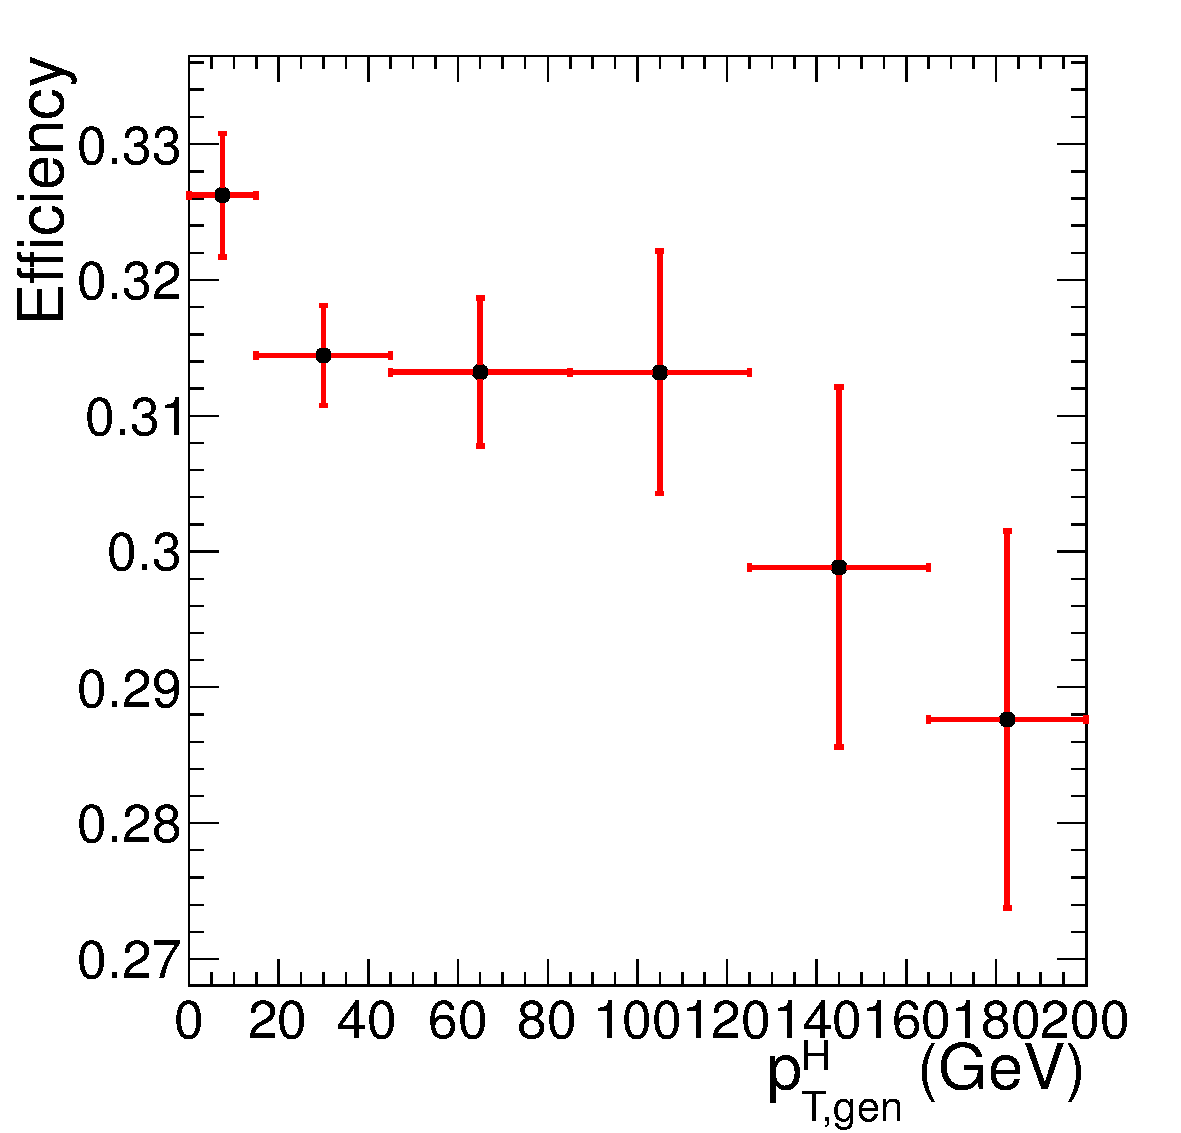
\includegraphics[width=0.45\textwidth]{images/eff_pth.pdf}
}
\subfigure[]{
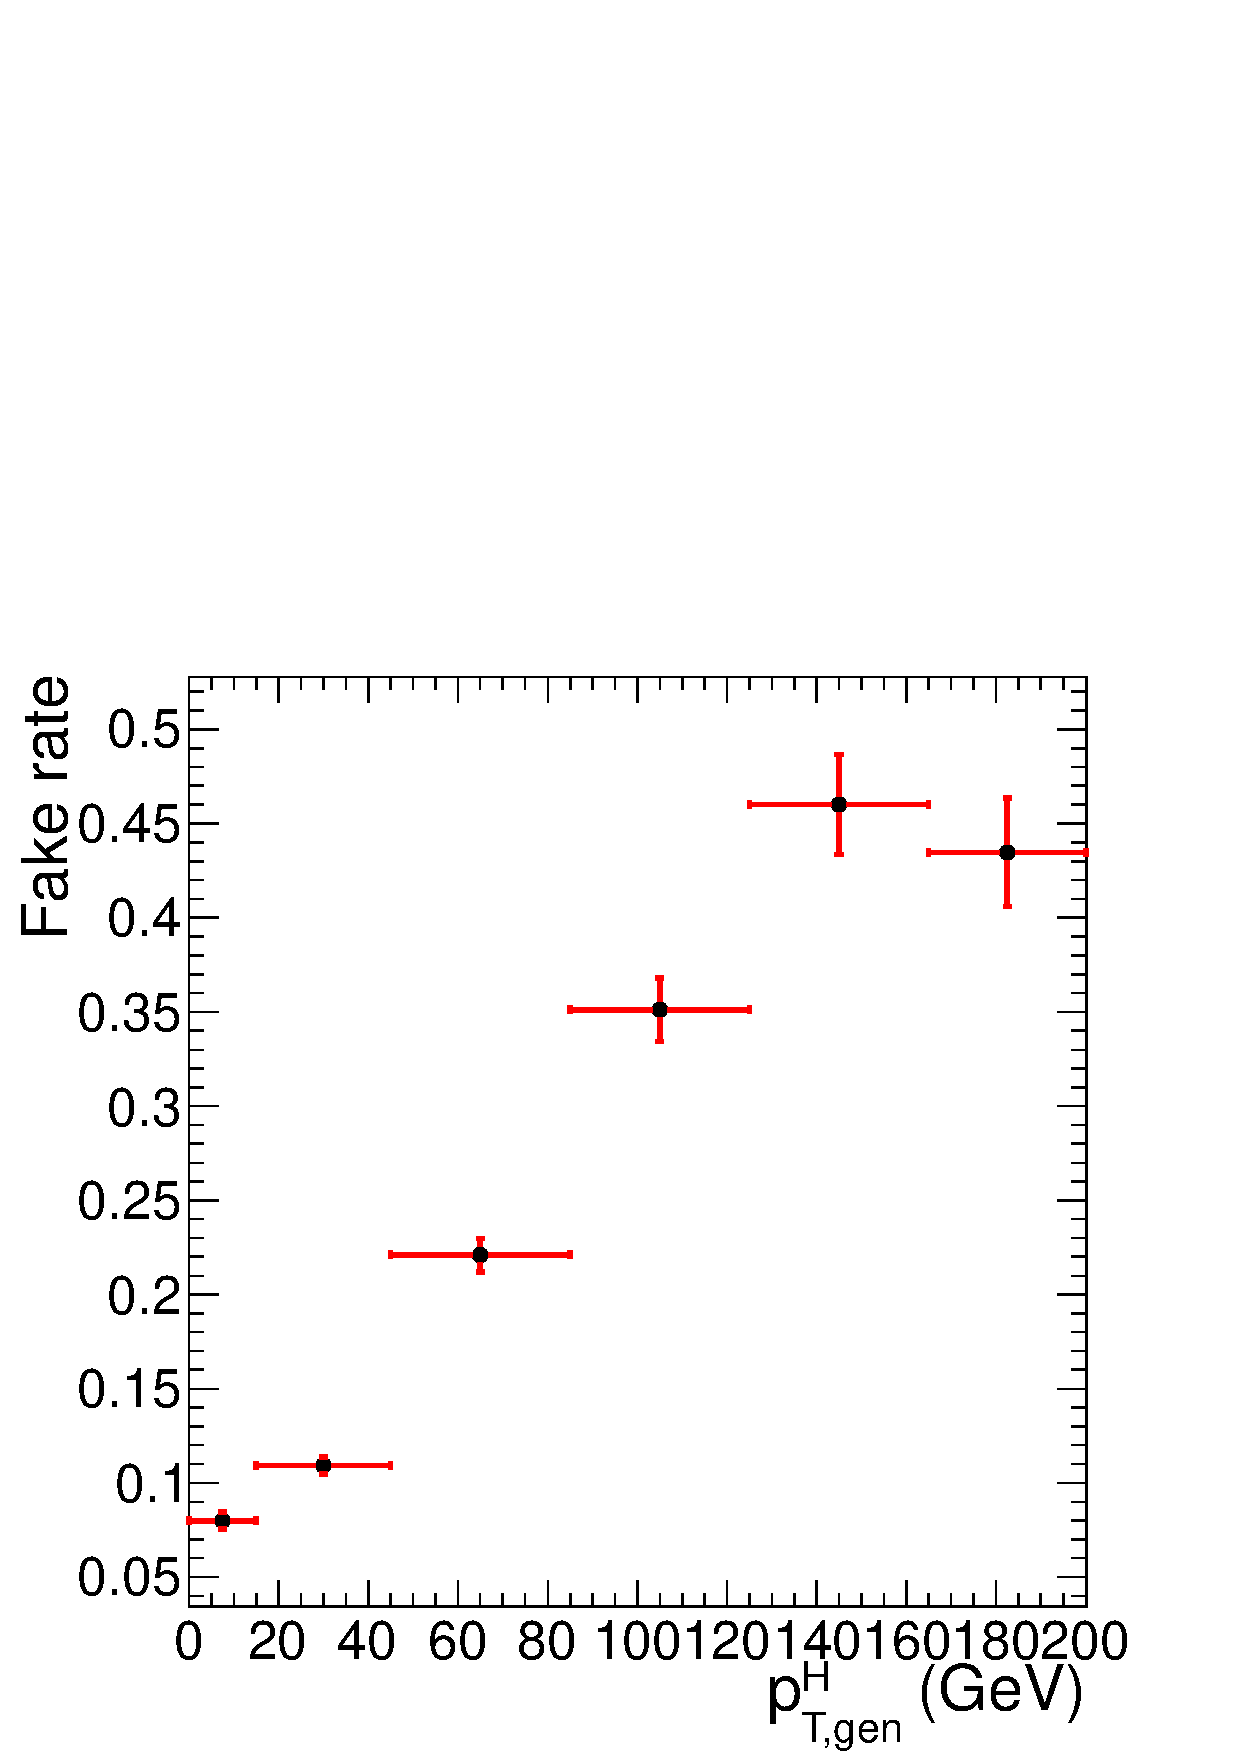
\includegraphics[width=0.45\textwidth]{images/fake_pth.pdf}
}
\caption{Efficiency of the full selection (a) and fake rate (b) as a function of \pth.\label{fig:sel_eff}}
\end{figure}


If a $4\pi$ acceptance is defined, requiring just that the Higgs decays to WW and then to $2\ell2\nu$, the efficiency becomes $\epsilon=0.03960\pm{0.00033}$ and the fake rate is zero. 





